\documentclass[10pt]{beamer}

\usetheme{CambridgeUS}
\setbeamercolor{normal text}{bg=black!10}
\setbeamercovered{transparent}

\usepackage{graphicx}
\usepackage{color}
\usepackage{hyperref}
\usepackage{multimedia}

\usepackage{helvet}
\renewcommand{\familydefault}{\sfdefault}

\title{Introduction to ROS}
\subtitle{(Robot Operating System)}
\author{HMW-Alexander}
\date{2016-03-29}
\institute{Nagoya University}

\begin{document}
 
 \maketitle
 
 \section{Overview}
 
 \subsection{Contents}
 
 \begin{frame}{Contents}
  \begin{itemize}
   \item {\bf{Introduction}}
   \begin{itemize}
    \item What is ROS?
    \item Why do we need ROS?
    \item How does ROS Work?
   \end{itemize}
   \pause
   \item {\bf{Getting Started with ROS}}
   \begin{itemize}
    \item Turtle Example
    \item Basic Operations
   \end{itemize}
   \pause
   \item {\bf{Practice}}
   \begin{itemize}
    \item 2D LiDAR and SLAM
    \item Data Collection\footnote{No real practice, we will use bag data for instead.}, Visualization and Processing
   \end{itemize}
  \end{itemize}
  \pause
  \begin{block}{The Goal of This Course}
   \begin{itemize}
   \item Know why we need ROS.
   \item Know how ROS works.
   \item Know basic operations to play with ROS.
   \end{itemize}
  \end{block}
 \end{frame}
 
 \subsection{Reference}
 
 \begin{frame}{Reference}
  \begin{itemize}
   \item {\bf{ROS Documentation}}: \url{http://wiki.ros.org}
   \item {\bf{ROS Introduction Lecture}}: Real-world data circulation science leader human resource development program
   \item {\bf{"A Gentle Introduction to ROS"}} -- Jason M. O'Kane.
   \item {\bf{"Learning ROS for Robotics Programming"}} -- Aaron Martinez \& Enrique Fernández
  \end{itemize}
 \end{frame}

  \begin{frame}{}
  \begin{center}
   \LARGE Introduction
  \end{center}
 \end{frame}
 
 \section{Introduction}
 
 \begin{frame}{ROS: Five Years (Video)}
  \movie[width=\textwidth,height=0.8\textheight,autostart,showcontrols]{
\includegraphics[width=\textwidth]{ROS.png}}{ROS- Five Years.mp4}
 \end{frame}
 
 \subsection{What is ROS?}
 
 \begin{frame}{What is ROS (Robot Operating System)?}
   \begin{block}{A meta-operating system for robot software development}
    \begin{itemize}
     \pause
     \item {\bf{Partly based on a "real" operating system}}
     \begin{itemize}
      \item processes management system
      \item file system
      \item user interface
      \item programming utilities (compiler, threading model, etc.)
     \end{itemize}
     \pause
     \item {\bf{A meta-operating system}}
     \begin{itemize}
      \item built on the top of an operating system
      \item works alongside an operating system
      \item allows different processes to communicate with each other at runtime
     \end{itemize}
     \pause
     \item {\bf{A framework for robot software development}}
     \begin{itemize}
      \item easily share a piece of software with other robots [philosophy of ROS]
     \end{itemize}
    \end{itemize}
   \end{block}
 \end{frame}
 
 \begin{frame}{What is ROS (Robot Operating System)?}
  \begin{block}{ROS is not...}
   \begin{itemize}
    \pause
    \item {\bf{is not a programming language}}
    \begin{itemize}
      \item ROS programs are routinely written in C++.
      \item client libraries are also available for Python, Java, Lisp, etc.
    \end{itemize}
    \pause
    \item {\bf{is not only a library}}
    \begin{itemize}
      \item ROS also includes a central server, a set of command-line tools, a set of graphical tools, and a build system.
    \end{itemize}
    \pause
    \item {\bf{is not an integrated development environment}}
    \begin{itemize}
      \item ROS can be used with most popular IDEs.
    \end{itemize}
   \end{itemize}   
  \end{block}
 \end{frame}

 
 \begin{frame}{Why do we need ROS?}
  \begin{block}{Programming in Your CS courses}
   \begin{itemize}
    \item Seldom run two or more programs simultaneously.
    \item Seldom make programs that talk to each other.
    \item Seldom consider letting others take an advantage of your programs.
   \end{itemize}
  \end{block}
  \pause
  \begin{block}{Before ROS}
   \begin{itemize}
    \item It is very hard to realize {\em{inter-communication}} and {\em{extensibility}} by raw APIs from operate system directly
   \end{itemize}
  \end{block}
  \pause
  \begin{block}{After ROS}
   \begin{itemize}
    \item Hierarchical abstraction and management of running programs
    \item Universal communication between programs
    \item A collection of powerful programs and code libraries as extension.
   \end{itemize}
  \end{block}
 \end{frame}
 
 \begin{frame}{How does ROS work? (Three levels of ROS)}
 
 \begin{block}{File System Level}
  \begin{itemize}
   \item package, manifest, message types
   \item An organization of the ROS related files (application, manifest, definition)
  \end{itemize}
 \end{block}
 \begin{block}{Computation Graph Level}
  \begin{itemize}
   \item node, master, parameter server, message, topic, bag
   \item The graph model and architecture of ROS
  \end{itemize}
 \end{block}
 \begin{block}{Community Level}
  \begin{itemize}
   \item distribution, repository, The ROS Wiki, etc..
   \item The resources from Internet
  \end{itemize}
 \end{block}  
 \end{frame}

 \begin{frame}[allowframebreaks]{How does ROS work? (Basic Concepts)}
  \begin{block}{Package}
   \begin{itemize}
    \item all ROS software is organized into packages
    \item a coherent collection of executable and supporting files
   \end{itemize}   
  \end{block}
  \begin{block}{Manifest}
   \begin{itemize}
    \item a "package.xml" file
    \item defines some details about the package:
    \begin{itemize}
     \item name, version, maintainer, dependencies
    \end{itemize}
   \end{itemize}
  \end{block}
  \begin{block}{Message Type}
     \begin{itemize}
      \item define the type of message in the communication within ROS
     \end{itemize}
    \end{block}
 \begin{block}{Node}
  \begin{itemize}
   \item a running instance of a ROS program
  \end{itemize}
 \end{block}
 \begin{block}{Master}
  \begin{itemize}
   \item enable the communications of a collection of independent nodes
  \end{itemize}
 \end{block}
 \begin{block}{Parameter Server}
  \begin{itemize}
   \item a central location to store parameters for nodes
  \end{itemize}
 \end{block}
 \framebreak
 \begin{block}{Message}
  \begin{itemize}
   \item nodes communicate with each other through messages
   \item a message contains data
   \item pre-defined and user-defined message types
  \end{itemize}
 \end{block}
 \begin{block}{Topics}
  \begin{itemize}
   \item each massage must have a name to be routed by the ROS network
   \item node is sending data = node is publishing a topic
   \item node is receiving data = node is subscribing a topic
  \end{itemize}
 \end{block}
 \begin{block}{Bags}
  \begin{itemize}
   \item a universal format to save and play back ROS message data
  \end{itemize}
 \end{block}
 \end{frame}
 \begin{frame}{How does ROS work?}
 
 \begin{block}{How does ROS work}
 \begin{itemize}
   \item ROS architecture is based on the graph-model
   \item the node of the graph is an instance of software
   \item the edge of the graph is the message communication route
   \item the master of ROS maintains the many-many communication
 \end{itemize}
 \end{block} 
 \begin{center}
  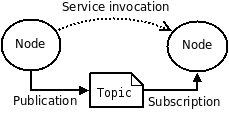
\includegraphics[width=0.5\textwidth]{graph-model.png}
 \end{center}

 \end{frame}

 \begin{frame}{}
  \begin{center}
   \LARGE Getting Started with ROS
  \end{center}
 \end{frame}
 
 \section{Getting Started with ROS}
 \subsection{Architecture with Turtle Example} 
 
 \begin{frame}{Architecture with Turtle Example}
  \begin{block}{Starting turtlesim}
   \begin{itemize}
    \item roscore
    \item rosrun turtlesim turtlesim\_node
    \item rosrun turtlesim turtle\_teleop\_key
   \end{itemize}
  \end{block}
  \begin{center}
   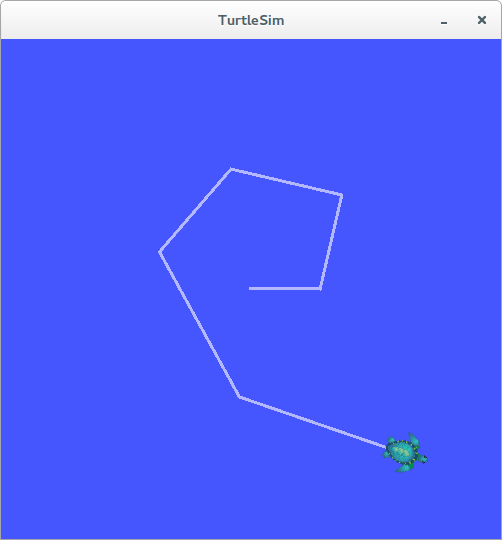
\includegraphics[width=0.35\textwidth]{turtlemove.png}~~
   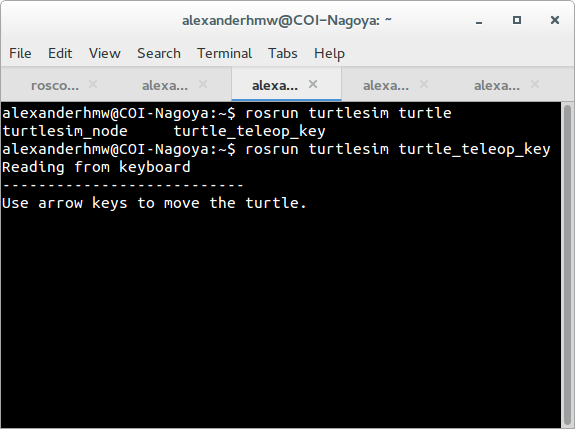
\includegraphics[width=0.35\textwidth]{turtlecontrol.png}
  \end{center}  
 \end{frame}
 
 \begin{frame}{Architecture with Turtle Example}
  \begin{block}{Check ROS Graph-model, Topics and Messages}
   \begin{itemize}
    \item rqt\_graph
    \item rostopic list
   \end{itemize}
  \end{block}
  \begin{center}
   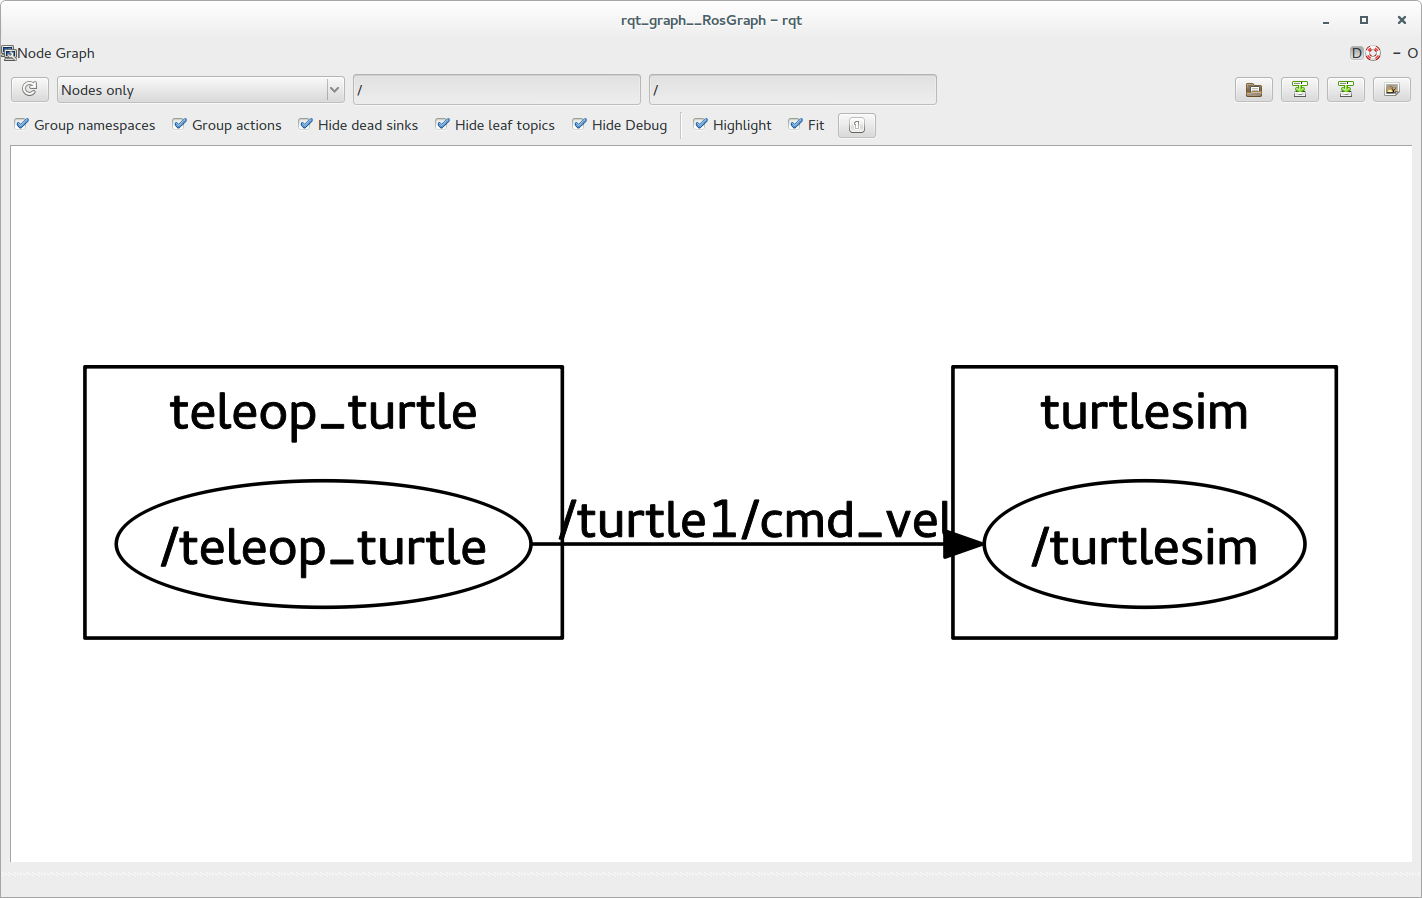
\includegraphics[width=0.4\textwidth]{rosgraph.png}~~
   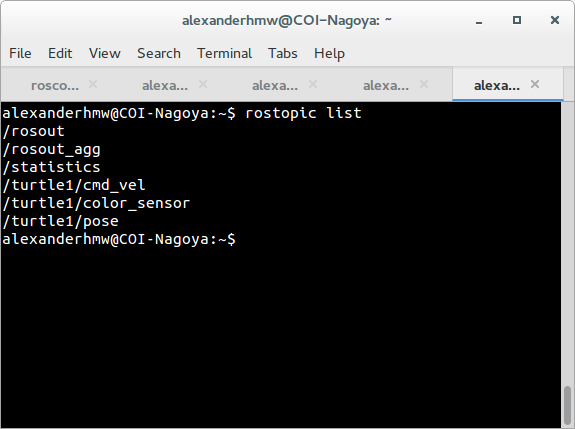
\includegraphics[width=0.4\textwidth]{rostopics.png}
  \end{center}
 \end{frame}
 
 \subsection{Basic Operation}
 
 \begin{frame}[allowframebreaks]{Basic Operation}
  \begin{block}{Navigating through the ROS filesystem}
   \begin{itemize}
    \item Find package's location: rospack find turtlesim
    \item List the files inside a package: rosls turtlesim
    \item Go to the package's folder: roscd turtlesim
   \end{itemize}
  \end{block}
  \begin{block}{Creating an ROS package}
   \begin{itemize}
    \item catkin\_create\_pkg hokuyo\_test std\_msgs rospy roscpp
    \item catkin\_create\_pkg [package\_name] [depend1] [depend2] [depend3]
   \end{itemize}
  \end{block}
  \begin{block}{Playing with ROS nodes}
   \begin{itemize}
    \item start master: roscore
    \item rosnode command: rosnode [param] -h
    \item launch node: rosrun [package] [executable] [ARGS] \\ rosrun turtlesim turtlesim\_node
   \end{itemize}   
  \end{block}
  \begin{block}{Interact with Topics and Messages}
   \begin{itemize}
    \item rostopic list: list the active topics
    \item rostopic echo: print messages to the screen
    \item rostopic info: print information about active topics
    \item rostopic type: print the topic message type
    \item rosmsg show: print the message fields
    \item rostopic pub: publish message to the topic \\
    rostopic pub -r 1 /turtle1/cmd\_vel geometry\_msgs/Twist '[1,0,0]' '[0,0,1]'
   \end{itemize}
  \end{block}
  \begin{block}{Using the Parameter Server}
   \begin{itemize}
    \item rosparam set parameter value: set the parameter
    \item rosparam get parameter: get the parameter
    \item rosparam load file: load parameters from the file
    \item rosparam dump file: dump parameters to the file
    \item rosparam delete parameter: delete the parameter
    \item rosparam list: list the parameter names
   \end{itemize}
  \end{block}
  \begin{block}{Some Useful Tools}
   \begin{itemize}
    \item rqt\_graph: display graph-model
    \item rviz: visualization tool
   \end{itemize}
  \end{block}
 \end{frame}

    \begin{frame}{}
  \begin{center}
   \LARGE Practice
  \end{center}
 \end{frame}
 
 \section{Practice}
 
 \subsection{2D LiDAR and SLAM}
 
  \begin{frame}{2D LiDAR and SLAM (Video)}
  \movie[width=\textwidth,height=0.8\textheight,autostart,showcontrols]{
\includegraphics[width=\textwidth]{ROS.png}}{slam.mp4}
 \end{frame}
 
 \begin{frame}[allowframebreaks]{2D LiDAR and SLAM}
  \begin{block}{2D LiDAR}
   A set of horizontal laser beams are emitted for range detection.
   \begin{center}
    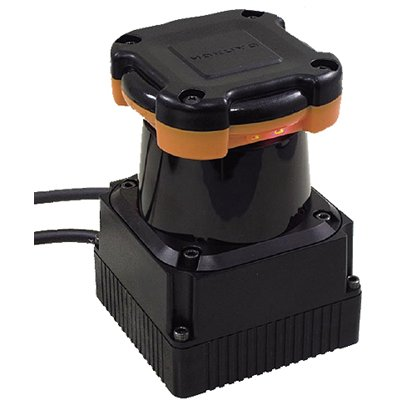
\includegraphics[height=0.3\textheight]{Hokuyo.jpg}
    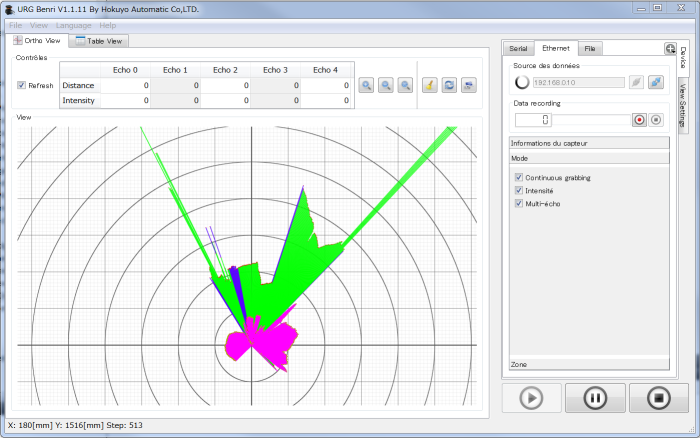
\includegraphics[height=0.3\textheight]{UrgBenri_screenshot.png}
   \end{center}
  \end{block}
  \begin{block}{SLAM}
   Simultaneous Localization and Mapping
  \end{block}
  \begin{block}{Graph-Model}
   \begin{center}
    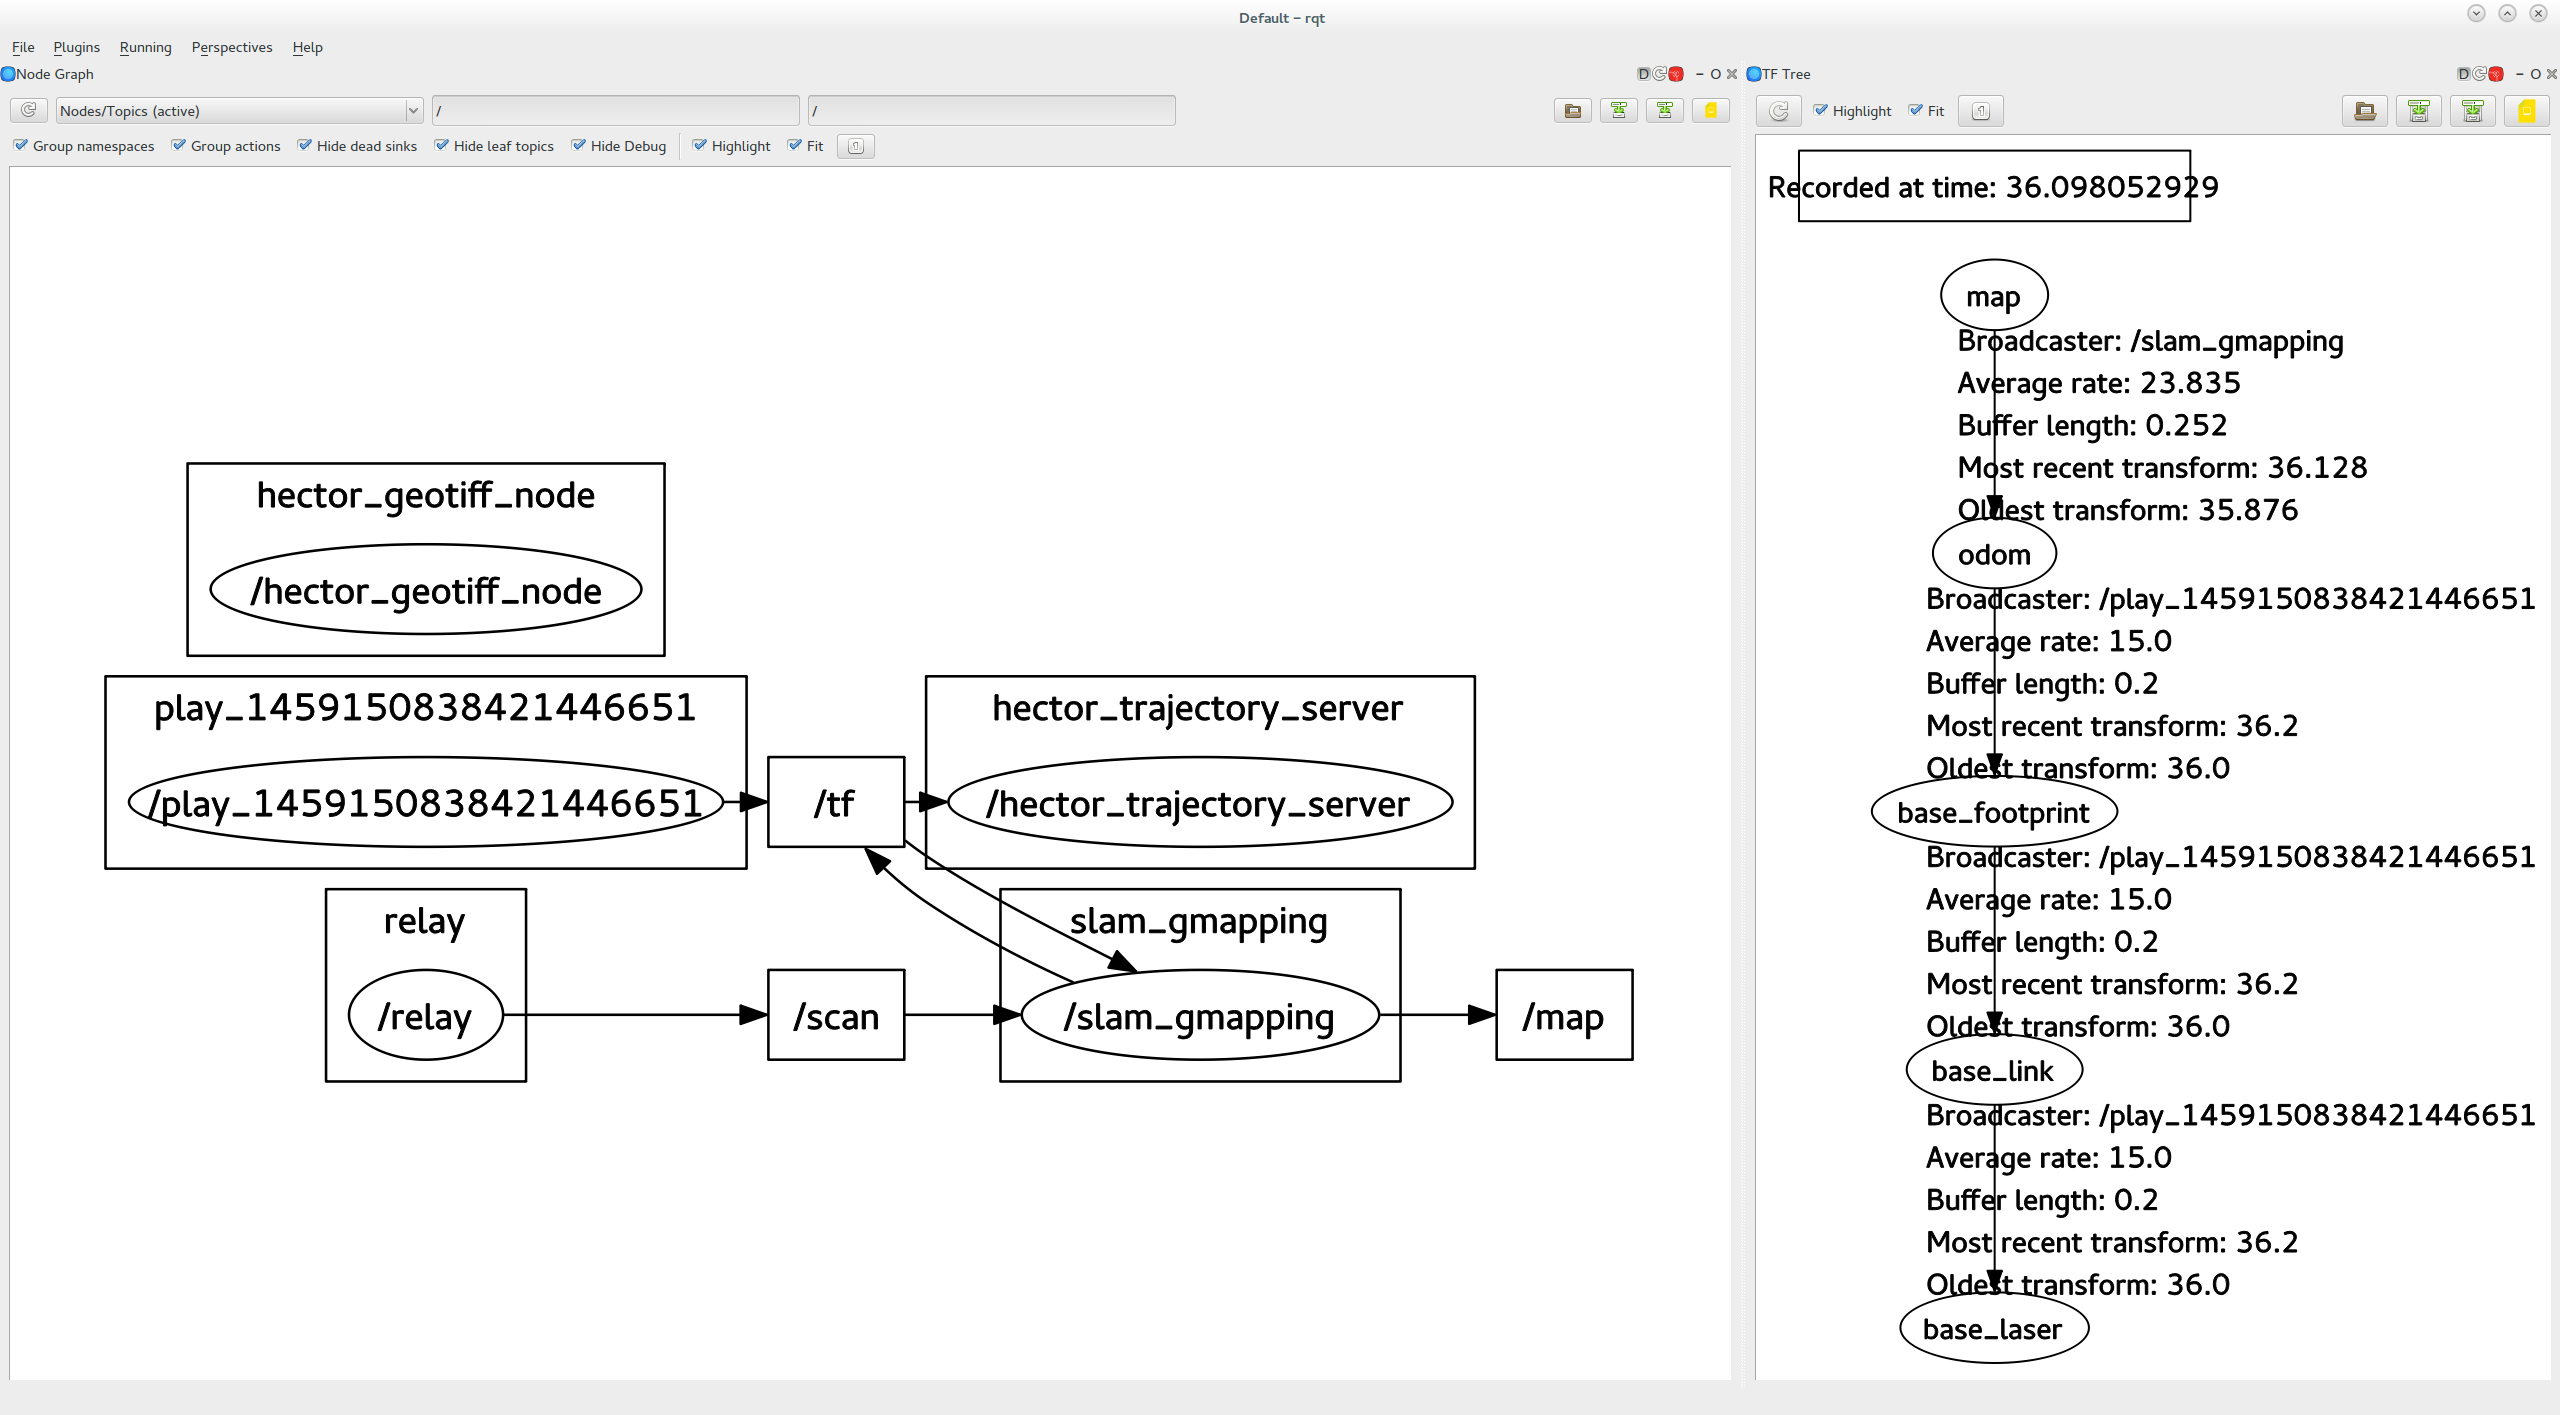
\includegraphics[width=1\textwidth]{graph-tf.png}
   \end{center}
  \end{block}
 \end{frame}

 \subsection{Data Collection, Visualization and Processing}
 \begin{frame}[allowframebreaks]{Data Collection, Visualization and Processingg}
  \begin{block}{Preparation}
   \begin{itemize}
    \item Install external libraries:
    \begin{itemize}
	    \item sudo apt-get install ros-hydro-gmapping [ros-hydro-hokuyo-node]
    \end{itemize}
    \item Build a workspace:
    \begin{itemize}
	    \item mkdir $\sim$/catkin\_ws/src
	    \item cd $\sim$/catkin\_ws/src
	    \item catkin\_init\_workspace
    \end{itemize}
    \item Create a package:
    \begin{itemize}
	    \item catkin\_create\_pkg hokuyo\_test std\_msgs rospy roscpp
	    \item copy the "launch" folder to path $\sim$/catkin\_ws/src/hokuyo\_test/
	    \item cd $\sim$/catkin\_ws
	    \item catkin\_make
	\end{itemize}
   \end{itemize}
  \end{block}
  \begin{block}{Test Package and create a "maps" folder}
	  	\begin{itemize}
	  		\item cd $\sim$/catkin\_ws
	  		\item source devel/setup.bash\footnote{Register the package to the system. In the following, you should execute this order when you open a new terminal.}
	  		\item roscd hokuyo\_test
	  		\item mkdir maps
	  	\end{itemize}
  \end{block}
  \begin{block}{Data Collection (No practice)}
   You can play with a Hokuyo laser scanner using the following orders.
   \begin{itemize}
    \item rosparam set hokuyo\_node/calibrate\_time false
    \item rosparam set hokuyo\_node/port /dev/ttyACM0
    \item sudo chmod a+rw /dev/ttyACM0
    \item rosrun hokuyo\_node hokuyo\_node
    \item rosbag record -o hokuyo /scan
   \end{itemize}
  \end{block}
  \begin{block}{Visualization of Hokuyo Data}
   \begin{itemize}
    \item roscore (if you don't start a master)
    \item rviz
    \item cd (the path holding hokuyo.bag)
    \item rosbag play hokuyo.bag $--$clock
   \end{itemize}
   \begin{center}
    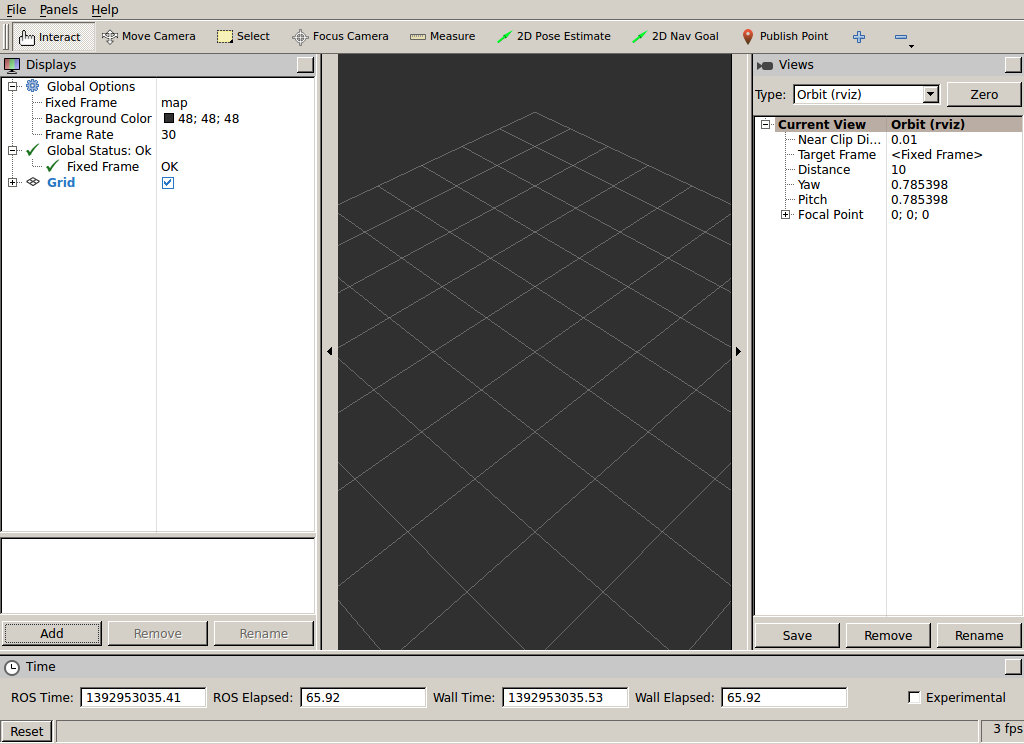
\includegraphics[width=0.3\textwidth]{rviz.png}~~
    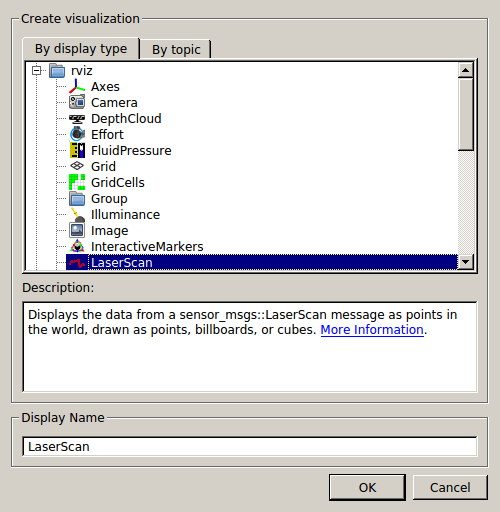
\includegraphics[width=0.3\textwidth]{topics.png}~~
    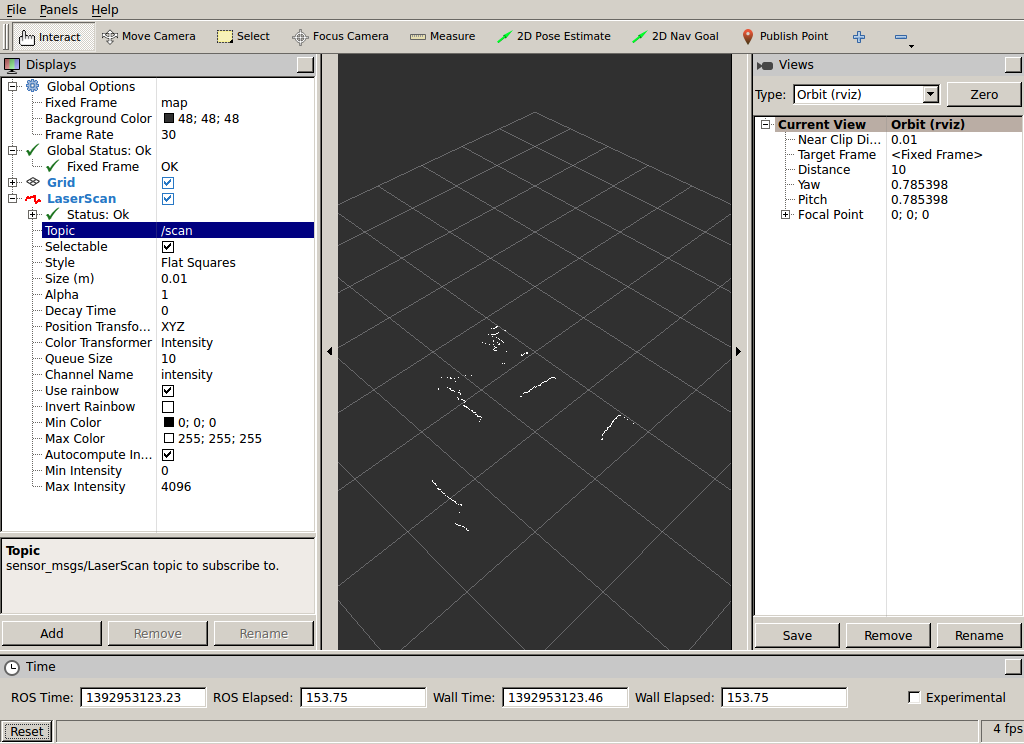
\includegraphics[width=0.3\textwidth]{scan.png}
   \end{center}
  \end{block}
  
  \begin{block}{Processing (SLAM)}
   \begin{itemize}
    \item roslaunch hokuyo\_test slam.launch
    \item rostopic pub syscommand std\_msgs/String "savegeotiff"
    \item roscd hokuyo\_test
    \item eog maps/hector\_slam\_map\_xx:xx:xx.tif
   \end{itemize}
   \begin{center}
    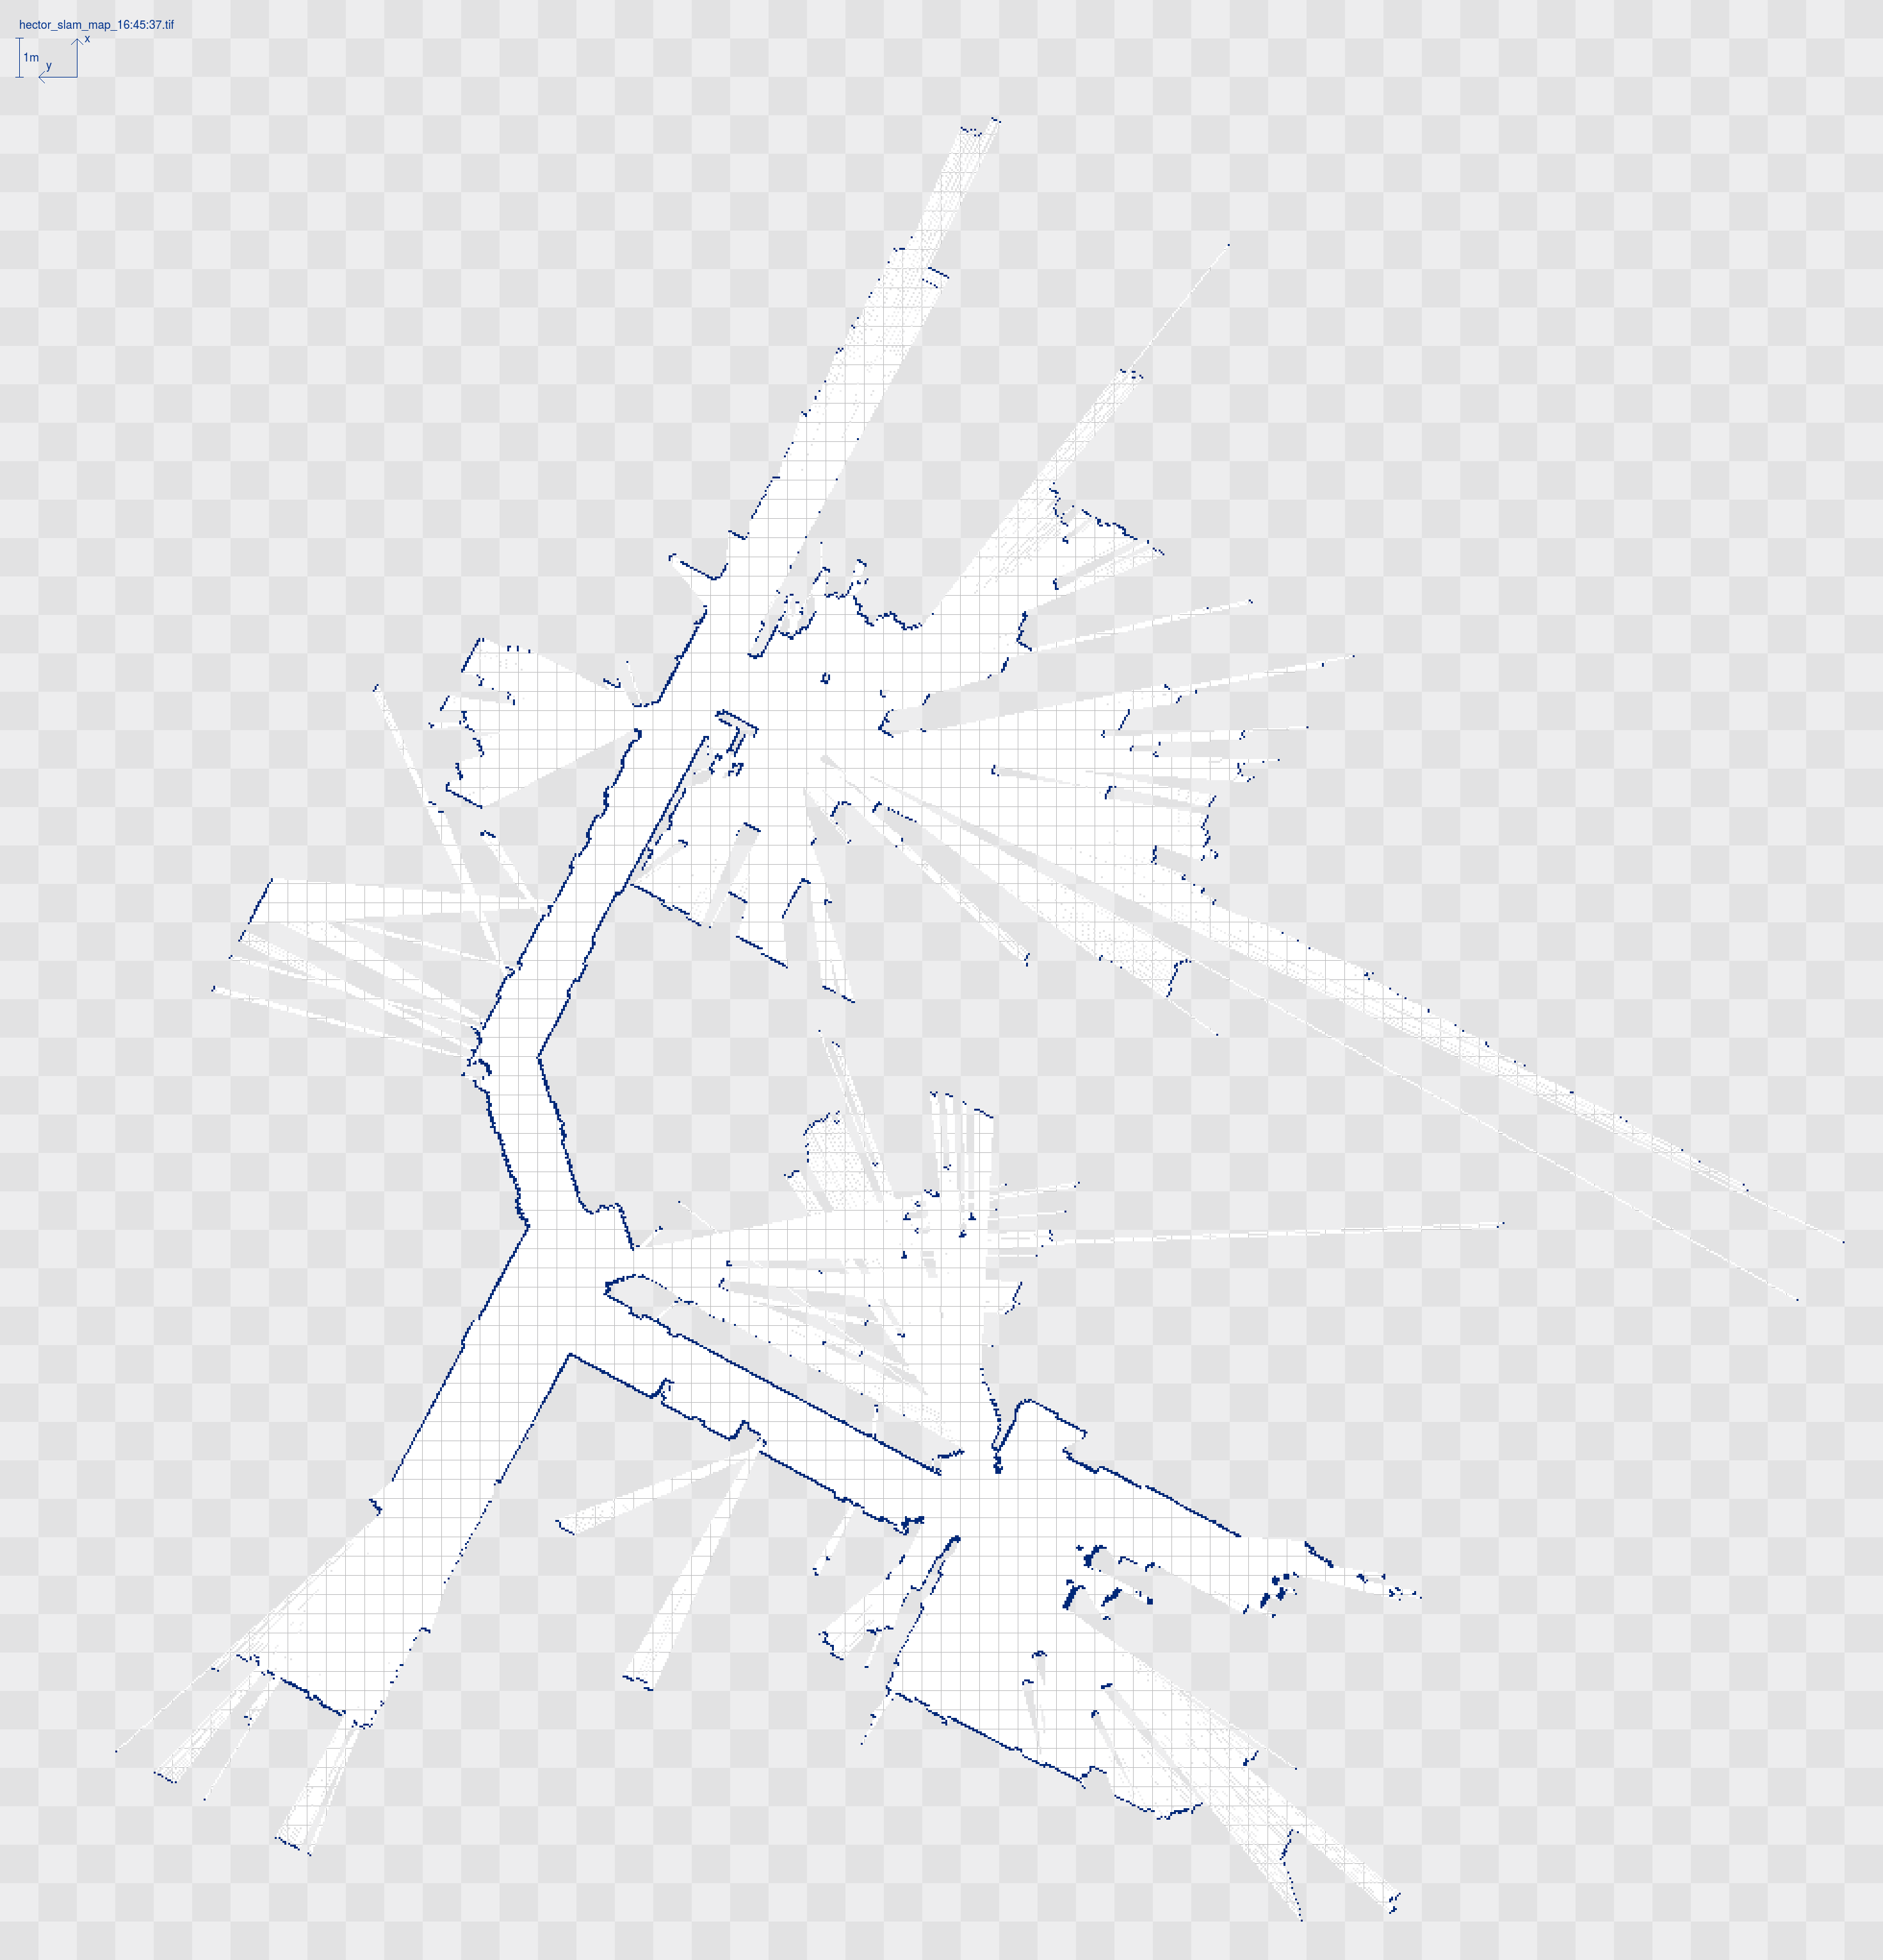
\includegraphics[width=0.3\textwidth]{newmap.png}
   \end{center}
  \end{block}  
 \end{frame}
 
 \section{Conclusion}
 
 \begin{frame}{Conclusion}
 \begin{block}{About ROS}
  \begin{itemize}
   \item ROS is a meta-operation system for the robot software development
   \item Easily realize inter-communication and extensibility of softwares
   \item ROS is based on graph-model
   \begin{itemize}
    \item Node is a software instance
    \item Edge is a message communication route
    \item Master maintains the many-many communication
   \end{itemize}
  \end{itemize}

 \end{block}
 
 \begin{block}{This Course}
  \begin{itemize}
   \item Play with Turtle Example
   \item Basic Operations
   \item Practice with 2D LiDAR Data and SLAM
   \item How to develop a node is not included in this course (see Reference)
  \end{itemize}
 \end{block}
 
 
 
 \end{frame}
 
     \begin{frame}{}
  \begin{center}
   \LARGE Thank you very much!
  \end{center}
 \end{frame}
 
\end{document}